
\section{Vehicles}
\label{sec:vehicles}

Since this is a traffic simulation, the traffic participators play a
heavy role in this simulation. Traffic participators can be anything
that uses a road, e.g.  cars, trucks, bicycles, even tramways. \\

\noindent In this project we limited ourselves to the cars. Figure 
\ref{fig:vehicles} shows the according classes. \\

\begin{figure}[H]
\begin{center}
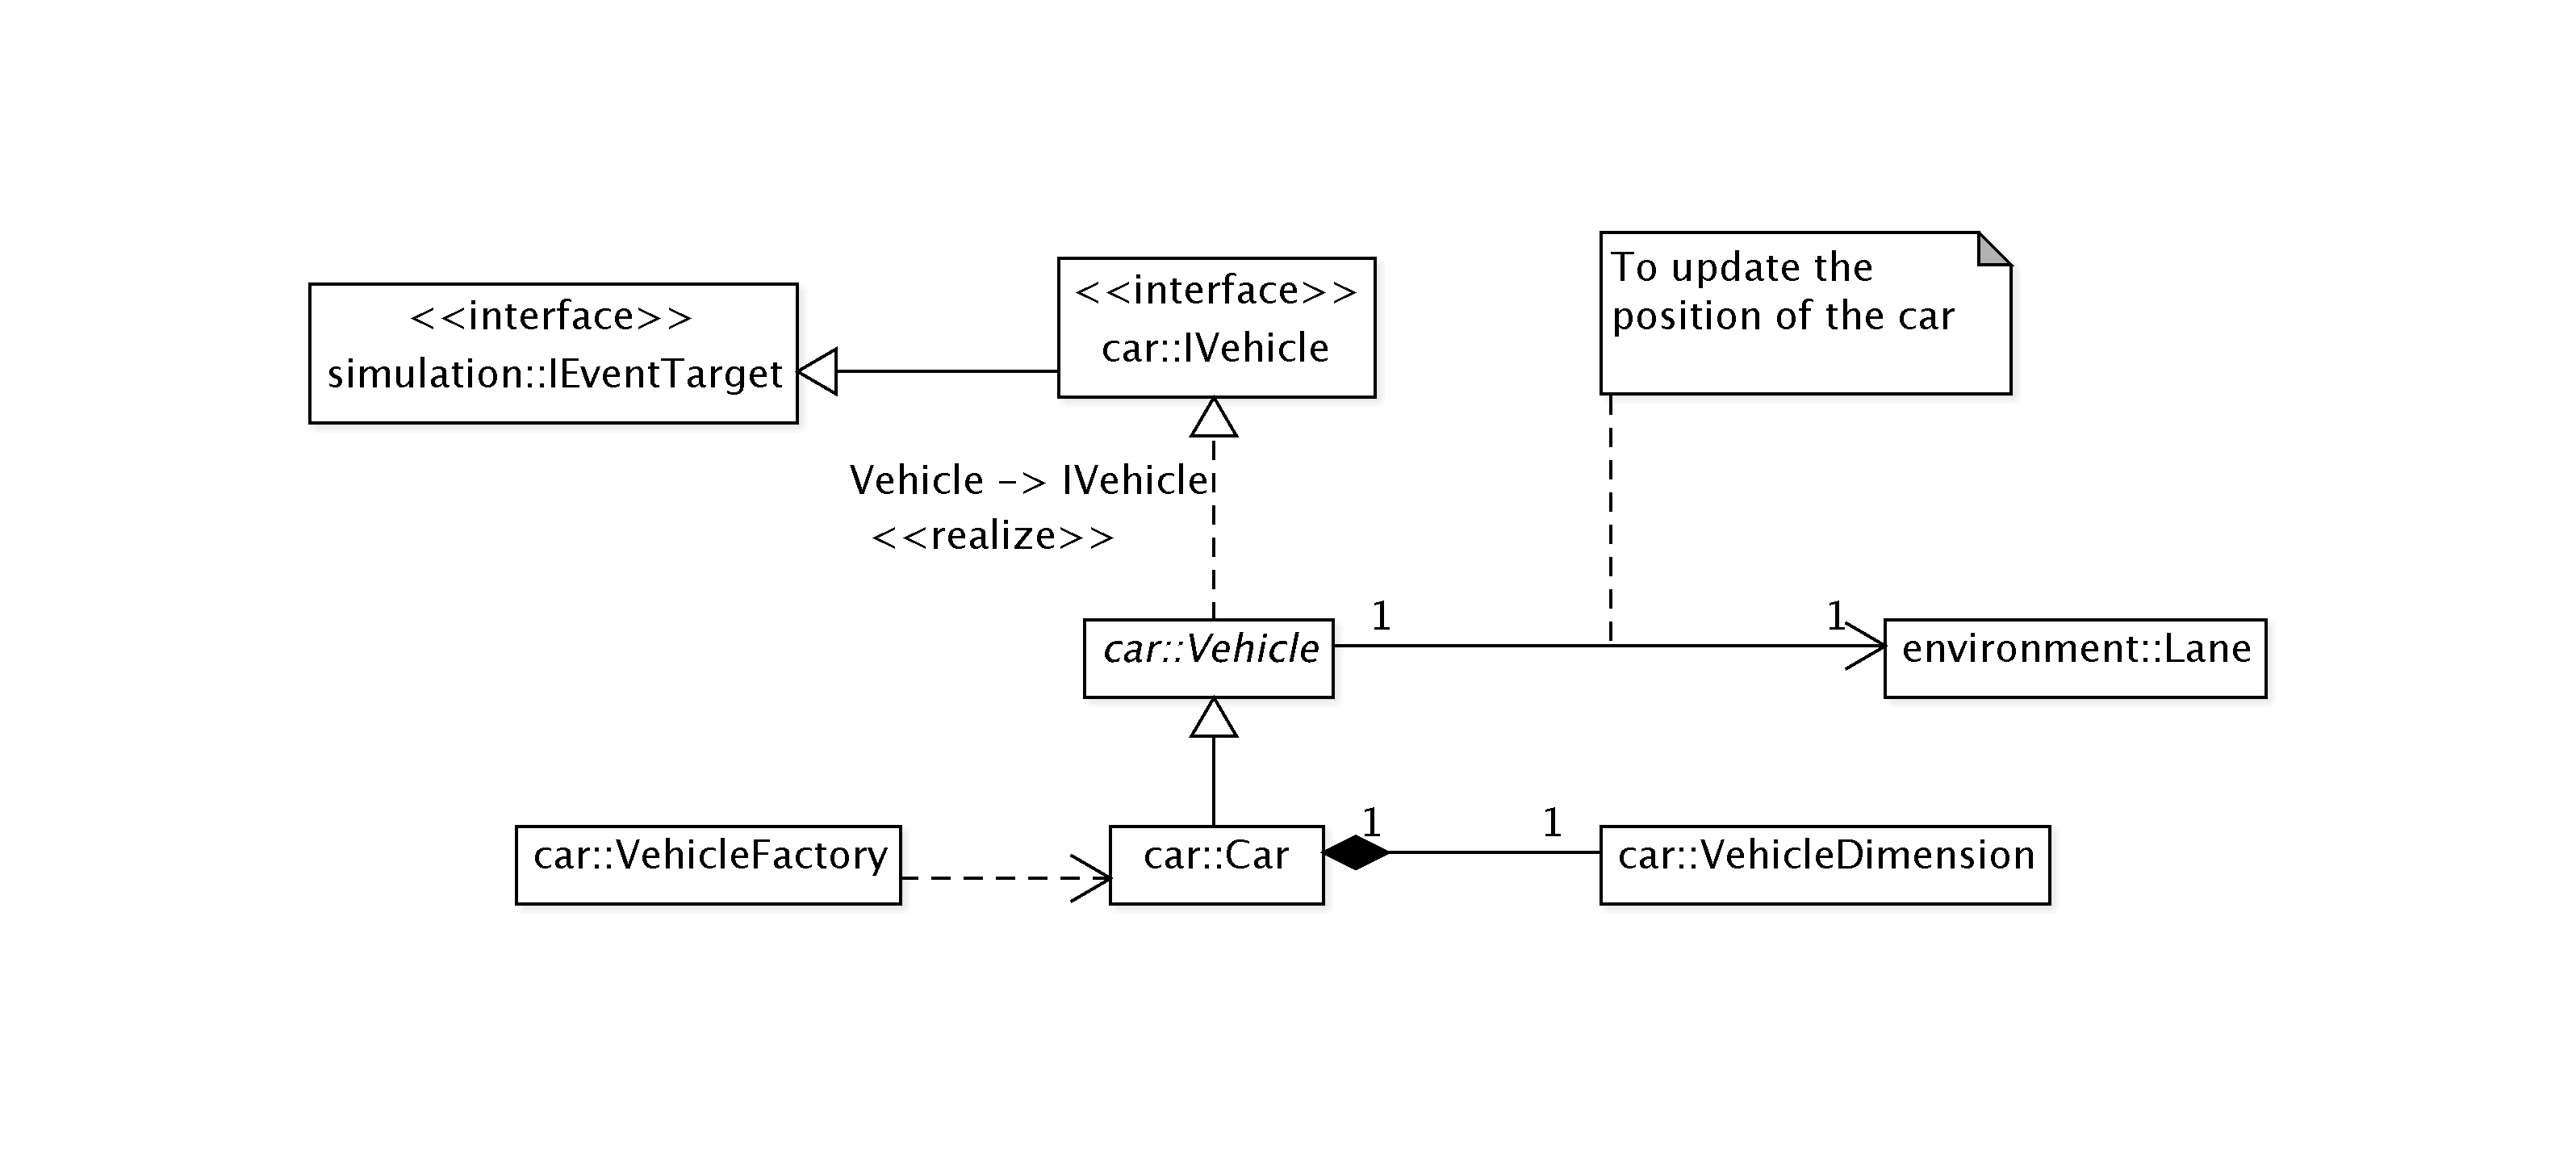
\includegraphics[width=\textwidth]{images/vehicles.png}
\end{center}
\caption{The composition of the vehicle objects}
\label{fig:vehicles}
\end{figure}

\subsection{Cars}

Cars are fairly easy objects in our world. Besides the obvious parameters
like position, current speed, current acceleration, maximal acceleration
and deceleration they also contain an object \emph{VehicleDimension} that
contains information about the dimensions of a vehicle. We implemented this
to achieve a high level of detail concerning the estimation of distances
by the driver. \\

In this simulation, the maximal acceleration and deceleration values
are chosen by random within some range to simulate different types of
cars. At this point of progress, the cars cannot reverse. We would have
to adjust the driver view concept (\ref{sec:driverView}) so that the
driver can see things that are behind him by either introduce mirrors
or turn the driver view over to the back of the vehicle.

\subsection{Driver's influence}
\label{sec:driverInfluence}

The only influence that the driver currently has on the vehicle is the 
acceleration. It can range from -1 (full braking) to 1 (full acceleration)
where 0 is to keep the current speed. These values are not applied directly,
instead the vehicle receives them as an event (\ref{sec:eventSystem}).

\subsection{Movement}

To update the position of the car while it's moving around, it is given
a time stamp from the simulation (\ref{sec:simulation}) that indicates 
the elapsed time. Based on the current speed and acceleration of the 
vehicle, the driven distance is calculated. This distance is then passed
to the lane, which calculates the new absolute position in the world. \\

\noindent The current speed is calculated by the basic equation for
acceleration: \\

$ v = v_0 + a * t$ \\

\noindent where the acceleration can also be negative to simulate braking.
Similarly, the driven distance is calculated by \\

$ s = s_0 + v * t $ \\

TODO: is this correct??

\noindent In this process, the direction of the car and therefore the driver
view are updated too, in case the car moves around a curve. \\

\noindent Additionally the position of the moving way point has to be updated.

\subsection{Steering}
\label{sec:steering}

To make the simulation simpler, we decided to constrain ourselves regarding
the steering of the vehicles. Currently they can not move around quite freely, 
instead they drive on the lanes like they were on rails. This frees the 
driver from having to decide, in which direction she has to steer.

\subsection{Lane changes}
\label{sec:laneChanges}

Due to the configuration of the world, lanes can only connect to junctions
(\ref{sec:junctions}). In the process of driving through a junction, the 
junction offers the driver the possibilities to driver through. Once decided,
the lane that connects to the next road and the lane on that road are put 
into a queue in the according order. When the car reaches the end of a lane, 
it dequeues a lane from the queue and drives on on that lane.

